\section{Guest Client}\label{section:imp:guest}

This section covers the relevant implementation details of the guest-client web application. First, the storage mechanisms used to reduce data loading times are discussed, as well as their benefits and limitations. The latter part provides a closer look at the methods used from the BC.

\subsection{Storage Mechanisms}\label{subsection:frontend-storage-mechanism}

As introduced in Section \ref{chapter:technology}, the guest-client uses two technologies for data storage, the Vuex state management library and the Indexed Database (IDB). The guest-client includes a middle layer with wrappers for IDB that handle storage operations and the required logic to only fetch data from the BC when there is something new to display. 

\subsubsection{Cold Start}

When the application is first started up (Cold Start), the SC addresses of all available events are requested from the \textit{Event Factory} SC. From these, the application can retrieve the IPFS hash for the event's metadata, as well as for all ticket categories of the event. Using the provided hash, the metadata is then requested from IPFS. The application then builds a JavaScript Data-Object from the received data and stores it in the application state, as well as persists it in the IDB. The stored object contains information such as title, SC address, location, time of the event as well as information on the ticket categories such as price, supply, description, and seat-mapping.
In the same way, the application requests the Ethereum address of the user's wallet and creates a Data-Object for the user. This also initializes an empty ticket inventory. 
Each storage entity also contains a record \textit{lastFetchedBlock}, which represents the block number at which it has been updated last, which is set to the current block right before storing them in IDB.

During this initial data fetching phase the application is still usable and responsive, although there is no information on events displayed yet. When the data is loaded, the user receives a notification and all UI elements are populated, e.g. the list of events.
At this moment the user can interact with the application in its full scope. 

\subsubsection{Warm Start}

On later application starts, the IDB is queried for all event contract addresses received from the \textit{Event Factory} SC. If there is an entry for an address present, the application knows that it has already fetched the metadata from the BC. Thus only new events will require a full fetch. However as aforementioned, the metadata also includes information on the supply of tickets and the owned tickets of the user, which is subject of change. This means that the application needs a way of having the most up-to-date state of the SC at all time. The easiest way to ensure this would be to load the metadata for all events from their SC and IPFS hash also on warm starts. However, as further discussed in the evaluation (Chapter \ref{section:eval-preloading}), this is not feasible due to high loading times even with a low number of events.

This problem is solved using solidity events. SCs can emit events when one of their methods is invoked. These events contain an identifier (e.g. \textit{ticketBought}) and the relevant information, e.g. the buyers Ethereum address, the event contract address, and the ticket category. In most cases the client storage can be updated with only the information gathered from these events. These events are indexed with the block number of the BC at the time they were emitted.

On a warm start, the application requests all solidity events from the \textit{lastFetchedBlock}. For each type of solidity event, it assigns the correct handler and updates the data models according to the information in the received event. This procedure is also shown in the code snippet in Figure \ref{code:eventLoading}.

\begin{figure}[hbt]
    \lstinputlisting[language=Java]{code-snippets/loadEvents.js}
    \caption{Buying fungible tickets with affiliate addresses}
    \label{code:eventLoading}
\end{figure}

\paragraph{Example 1:} The client application receives an event of type \textit{ticketMetadata} which indicates that either a new ticket category has been created or the metadata of an existing category has been altered, resulting in an updated IPFS hash. Thus, the data loading logic checks if the ticket category exists within our data model and either updates or creates it with the new metadata from IPFS. From this point the application knows that it does not have to fetch data from IPFS for this ticket category again, except in case a new \textit{ticketMetadata} solidity event for the category is emitted. 

\paragraph{Example 2:} The application receives an event of type \textit{MintFungible} which indicates that some user has bought a ticket of a fungible ticket category. The application then decreases the amount of available tickets for this category in the data model. This type of event is also of interest for the user data model, since it might be the user of the local application who bought the ticket. Thus, the application also filters all solidity events of type \textit{MintFungible} by the buyer's address and updates the user's inventory if this is the case. This inventory is done with just the information available in the solidity event and does not lead any more interaction with the SC.

\subsubsection{Live Updates}

As described in the previous sections, the application fetches all data when it is served as either a conventional web page or a PWA. This however, can lead to incomplete data displayed to the user, if the user leaves the page open for an extended period of time without reloading it or in the case of an event with high demand and thus, a high number of people buying tickets concurrently. Also, if the user completes any action resulting in a different state of the BC himself (e.g. buying a ticket), the application should display this change immediately in order to prevent confusing the user on if the transaction actually succeeded. 

To address the latter issue, the application triggers minor data fetches similar to a \textit{warm start}. The difference here being that only the data that has been changed for sure is being updated.

\begin{figure}[hbt]
    \centering
    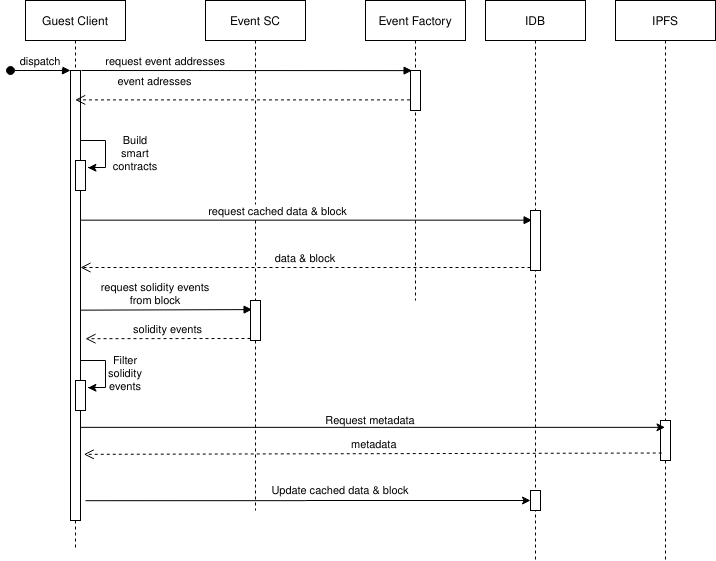
\includegraphics[width=14cm]{images/storage_sequence.png}
    \caption{Storage layer sequence diagram}
    \label{fig:storage_sequence}
\end{figure}

The bigger issue is posed by the former problem, where any BC state (e.g. number of tickets available for event x) can change at any point in time due to interactions originated from other users. In order to solve this problem there exist two main approaches. 

Firstly, the data loading logic can be triggered periodically in fixed time intervals. This requires experimental configuration of the time interval size in order to find the best trade-off between performance overhead for data fetching and out-of-date application state. 

The second approach is enabled by some functionality provided by the \textit{web3.js} library, which allows the subscription to specific Solidity events. The guest-client application also contains a small module to build these subscriptions for all relevant Solidity events upon application start. From this point on the application can assign the respective event handler for each Solidity event and react close to real time. This module is designed to be optional, since it does hurt the application's performance due to the high number of events which have to be subscribed to. Since the subscription functionality provided by \textit{web3.js} is designed in a non thread-blocking way, this implementation turned out to be easier on performance than the former method with fixed time intervals.
